\documentclass[english, 10pt]{article}
\usepackage[sexy]{evan}
% \usepackage{lstlang}
\usepackage{inconsolata}
\usepackage[shellescape]{gmp}
\usepackage{titlesec}
\usepackage{listings}
\usepackage{xcolor}
\allowdisplaybreaks%
\newcommand{\thiscoursecode}{CMSC 216}
\newcommand{\thiscoursename}{Introduction to Computer Systems}
\newcommand{\thisprof}{Prof. Nelson Padua-Perez}
\newcommand{\me}{Ekesh Kumar}
\author{Ekesh Kumar\thanks{Email: \mailto{0ekesh@gmail.com}}}
\newcommand{\thisterm}{Summer 2019}
\newcommand{\website}{http://www.cs.umd.edu/class/summer2019/cmsc216/}%chktex 8
\usepackage{ifpdf}
\ifpdf%
\DeclareGraphicsRule{*}{mps}{*}{}
\fi
% \listfiles
% \VerbEnvir{align tikzpicture algorithm}
%%%Headers
\lhead{\textbf{\me} \\ \textbf{\thisprof}}
\rhead{\textbf{\thiscoursename} \\ \textbf{\thisterm}}

% C Programs Listing
\lstdefinestyle{customc}{
  belowcaptionskip=1\baselineskip,
  breaklines=true,
  frame=L,
  xleftmargin=\parindent,
  language=C,
  showstringspaces=false,
  basicstyle=\footnotesize\ttfamily,
  keywordstyle=\bfseries\color{green!40!black},
  commentstyle=\itshape\color{purple!40!black},
  identifierstyle=\color{blue},
  stringstyle=\color{orange},
}


\definecolor{mGreen}{rgb}{0,0.6,0}
\definecolor{mGray}{rgb}{0.5,0.5,0.5}
\definecolor{mPurple}{rgb}{0.58,0,0.82}
\definecolor{backgroundColour}{rgb}{0.95,0.95,0.92}
 
\lstdefinestyle{CStyle}{
    backgroundcolor=\color{backgroundColour},   
    commentstyle=\color{mGreen},
    keywordstyle=\color{magenta},
    numberstyle=\tiny\color{mGray},
    stringstyle=\color{mPurple},
    basicstyle=\footnotesize,
    breakatwhitespace=false,
    breaklines=true,
    captionpos=b,
    keepspaces=true,
    numbers=left,
    numbersep=5pt,
    showspaces=false,
    showstringspaces=false,
    showtabs=false,
    tabsize=2,
    language=C
}


%%%%% TITLE %%%%%
\newcommand{\notefront}{%
\pagenumbering{arabic}
\begin{center}
{\small}
\textbf{\Huge{\noun{\thiscoursecode}}}
{\Huge \par}
{\Large{\noun{\thiscoursename}}}\\
\vspace{0.1in}
\vspace{0in}
\includegraphics[scale=0.3]{umd_cs.jpg} \\
\vspace{0.1in}{\noun\me} \\
{\noun\thisprof} \ $\bullet$ \ {\noun\thisterm} \ $\bullet$ \ {\noun{University of Maryland}} \\
{\ttfamily \url{\website}} \\
\end{center}
}

 \tikzstyle{class}=[
    rectangle,
    draw=black,
    text centered,
    anchor=north,
    text=black,
    text width=2cm,
    shading=axis,
    bottom color={rgb:red,222;green,222;blue,222},
    top color=white,shading angle=45]
%% End of

\begin{document}\thispagestyle{empty}
% \lstinputlisting[language=c]
  \notefront % IDK why it's giving error. ignore for now
  \tocandfigures
  
  \lstset{
  basicstyle=\footnotesize, frame=tb,
  xleftmargin=.2\textwidth, xrightmargin=.2\textwidth
}


% Change section headers
% \titleformat{\section}
%   {\Large\scshape}{\thesection}{1em}{}
% \titleformat{\subsection}
%   {\large\scshape}{\thesubsection}{1em}{}

%% End of setup.
% May
\section{Tuesday, May 28, 2019}
\subsection{Logistics}
\begin{enumerate}
\item All lectures are recorded and posted online.
\item No pop quizzes, no collaboration on projects.
\item Website sign-in: cmsc216/sprcoredump.
\item Office hours are immediately after class in IRB $2210$.
\item Everybody will get an Arduino -- this will be used later in the course. 
\item This class isn't curved.
\end{enumerate}

\newcommand{\ra}{\rightarrow}
\subsection{Basic Unix Commands}
Unix has lots of commands, but we want to first focus first on the ones that'll let us write and execute C programs. 
\begin{itemize}
    \item \verb!pwd! $\ra$  displays your current directory.
    \item \verb!ls! $\ra$ displays the files/directories in the current directory.
    \begin{itemize}
        \item \verb!ls -al! $\ra$ lists all of the files and directories, including hidden ones (Here, the \verb!a! flag functions to show hidden files, whereas the \verb!l! flag functions to list all entries with detailed information, like last date accessed). 
        \item \verb!ls -F! $\ra$ identifies directories by listing them with a $/$.
    \end{itemize}
    \item \verb!cd! $\ra$ change directory to the inputted parameter.
\end{itemize}
% Other easy unix stuff.  
% The 216 Public folder is where we'll be provided information
% Do work in the 216 folder.

% Set-up this:         /afs/glue/class/summer12019/cmsc/216/0101/public/bin/

\subsection{Introduction to C Programming}
In CMSC131 and 132, we learned Java. Unlike Java, C is not object-oriented; it has no concept of classes, objects, polymorphism, or inheritance. However, C can be used to implement some object-oriented concepts, like polymorphism or encapsulation. Consider the following program: 


\lstset{
caption=A First Program
}
\lstinputlisting[language=c]{may28/may2801.c}

How does this program work? 
\begin{itemize}
    \item The \verb!#include! allows the compiler to check argument types. It can compile without declaration, though the compiler will warn you. 
    \item Like Java, C provides a definition of the \verb!main()! function, where all C programs begin. 
    \item We return from \verb!main()! to end the program. For standard practice, we return $0$ to signal that everything worked out fine. 
\end{itemize}

Now, let's say we want to run this program. How can we do this? C programs need to be compiled before they can be executed. With the \verb!gcc! compiler, a very simple compilation command is \verb!gcc file.c!, from which we can run the executable by just typing $\verb!./file!$. 

Some more compilation options are summarized below (these are called \vocab{flags}): \begin{itemize}
    \item \verb!-g! enables debugging by generating and maintaining necessary symbols (e.g. line numbers) upon compilation.
    \item \verb!-Wall! warns about common things that might be a problem.
    \item \verb!-o filename! places an executable in the file name.
\end{itemize}
\section{Wednesday, May 29, 2019}
Last time, we analyzed a sample C program. It's important to know that returning $0$ in the \verb!main()! function is independent of the \verb!void! that appears in the main's header. That is, even if our header is \verb!int main(void)! instead of \verb!int main()!, we will still return $0$ at the end of the function. The \verb!void! is just an explicit way of telling our compiler that we shouldn't be passing any parameters in.

\subsection{More Unix Commands}
Some more Unix: \begin{itemize}
    \item The \verb!cp! command makes a copy of a file from a source to a destination. Some options are \verb!-a!, which allows us to preserve attributes, like timestamp modified. Also, \verb!-v! explains what's being done, while \verb!-r! copies recursively.   
    \item The \verb!-rm! command removes a file.
    \item The \verb!-mv! command renames a file or moves a file/directory to another directory. For example...
    \begin{itemize}
        \item \verb!-mv f1 f2! renames file \verb!f1! to \verb!f2!. 
        \item \verb!-mv f1 d1! moves the file \verb!f1! to the directory \verb!d1!.
        \item Finally, \verb!-mv d1 d2! moves the directory \verb!d1! to \verb!d2!.  
        \item The \verb!-cat! command displays the contents of a file.
    \end{itemize}
\end{itemize}
In Unix, we can create \vocab{aliases}, which are shortcut commands to use a longer command. Users can use the alias name to run the longer command while typing less. Without any arguments, the \verb!alias! command prints a list of defined aliases. A new alias is defined by assigning a string with the command to a name. We can add an alias by modifying the \verb!.aliases! file in the home directory of Grace. 

The general format for defining an alias is \verb!alias [alias name] 'command'!. So adding the line \verb!alias cookies 'ls'! would define the command \verb!cookies! to do the same thing as \verb!ls!

%sprcoredump

\subsection{Compilation Stages of a C Program}
C programs need to be compiled before they can be executed. What happens when we compile a C program? There are \vocab{three compilation stages}: \begin{enumerate}
    \item \textbf{Preprocessor Stage:} This stage is used to verify that program parts sees declarations that they need. Also, statements starting with a \verb!#! are called \vocab{directives} (for example, 
    \item \textbf{Translation:} In this stage, an object (\verb!.o!) file is created. In addition, the compiler checks to make sure that individual files are consistent with themselves.
    \item \textbf{Linkage:} Finally, this stage brings together one or more object files. It makes sure that the caller/calee to functions are consistent. The result is an executable file (by default, it's named \verb!a.out!), 
\end{enumerate}


\subsection{Variables in C}
There are a lot of data types in C, some of which include \verb!char, short, int, long int, float, double!, etc. In Java, data types take up the same amount of space, independent of the system they're run on. This is not true in C; the minimum size of various data types are not necessarily the same size on grace. We do not need to memorize the sizes of various data types; however, it is important to know that a \verb!char! data type is an exception to this rule: it always takes one byte. \\

Also unlike Java, there is no maximum size for a type; however, the following inequalities hold:
\begin{center}
\verb!sizeof(short)! $\leq$ \verb!sizeof(int)! $\leq$ \verb!sizeof(long)! \\[0.7em]
\verb!sizeof(float)! $\leq$ \verb!sizeof(double)! $\leq$ \verb!sizeof(long double)!
\end{center}

Suffixes allow us to specify a number of a given type. For instance, \verb!30000! is of type \verb!int!, whereas \verb!30000L! is of type \verb!long!.



In C, there is no default \verb!boolean! data types; anything with value $0$ is considered false, whereas any other value is considered true. However, we can use integers to represent booleans with \verb!true! mapping to $1$ and \verb!false! to $0$.

Consider the following code example:



\lstset{
caption=Conditional Example
}
\begin{center}
\lstinputlisting[language=c]{may29/may2901.c}
\end{center}

The print statement in conditional executes successfully for reasons described above.


\newpage












% garbage or trash
\section{Friday, May 31, 2019}

\subsection{printf() and scanf()}

When we're using \verb!printf()! to print something, we just print anything that's in the quotations. For instance, the line \verb!printf("Hello");! would print ``Hello,'' as we desire. 


To print variables, we use \vocab{conversion specifications}, which begin with the \verb!%!. These are just placeholders representing a value to be filled in during printed. More specifically, the \verb!%! \textit{specifies} how the value is \textit{converted} from its internal binary form to characters. For instance, the conversion specification \verb!%d! specifies that \verb!printf! is to convert an \verb!int! value from binary to a string of decimal digits. In summary,
\begin{itemize}
    \item \verb!%d! for integers,
    \item \verb!%c! for chars,
    \item \verb!%f! for floats,
    \item \verb!%s! for strings (null-terminated char array)
    \item \verb!%x! for hexadecimal form
    \item \verb!%e! for exponential form
    \item \verb!%u! for unsigned integer.
\end{itemize}

For example, the following code segment will print \verb!i = 10!. 

\lstset{
caption=Printing a Variable
}
\begin{center}
\lstinputlisting[language=c]{may31/may3101.c}
\end{center}



\verb!scanf()! is used for user input and it works similarly. The  introduce the \vocab{address} operator, which is denoted by a \verb!&!. The address operator is a unitary operator which, as its name specifies, returns the memory address of the variable on which it is acting on. When \verb!scanf()! is called, it starts processing the information in the inputted string, from left to right. For each conversion specification in the format string, \verb!scanf()! attempts to locate an item of the appropriate type in the input data, skipping any blank space if necessary. \\


Here's an example:


\lstset{
caption=Reading Variables
}
\begin{center}
\lstinputlisting[language=c]{may31/may3102.c}
\end{center}

Now suppose that the user enters the line \begin{center}
\verb!1 -20 .3 -4.0e3!.
\end{center}
The code above will convert its characters to the numbers they represent and assign the values $1, -20, 0.3, -4000.0$ to the four variables. 


Finally, one should keep in mind that \verb!char! variables are actually just integers that map to an ASCII character. So something like \verb!printf("%c", 65)! works completely fine; it prints the character \verb!A!. \\

% \subsection{Scanf() and}
There are two important things that one should check when using \verb!scanf()! and \verb!printf()!: \begin{enumerate}
    \item Check that the conversion specifications match the number of input variables and that each conversion is appropriate for the corresponding variable (as should also be done with \verb!printf()!. Since the compiler doesn't necessarily have to check for mismatches, there won't be any warning.
    \item Another trap involves the \verb!&! symbol, which should precede each variable in a \verb!scanf! call. Forgetting to put it can lead to unpredictable results. It is wrong to use the address-of operator in a printf() statement. 
\end{enumerate}

% A char is an integer!

A \vocab{segmentation fault} error occurs when the program attempts to access an area of memory that it should not be accessing. Why is it called a segmentation fault? Because the content of memory at the time of crash is stored into a \vocab{core file.}


We can get segmentation faults when using \verb!scanf()! or \verb!printf()! if we try to read into or print some variable that we don't have access to. 


% There are some more problems that can occur with \verb!scanf()! and \verb!printf()!.



% A scanf starting with \n.




\subsection{Control Statements}
C has \verb!if/else, for, do-while,! and \verb!switch! statements, just like in Java. But due to the compiler flags in our submit server, we won't be allowed to declare variables in the \verb!for loop! header. 

There's also \verb!break! and \verb!continue!, but they are bad practice and shouldn't be used often.


\subsection{Functions}
C functions have the following format to create a function \verb!returnType functionName(parameter list) { ... }! Just like in Java, to call a function, we just write \verb!functionName(argument list);!. 

However, if the function appears after the main, then we need to do something called \vocab{function prototyping}, which is just declaring the function before the main. This isn't necessary if we implement the function before the main, though. Function prototypes don't actually need the name of the variable, but it's easier to read with them.


In C, variables are passed in \textbf{by value}. This is different from Java, in which variables are passed in by reference. Some other things that are similar/different are: \begin{itemize}
    \item We can have recursion in C.
    \item We can \textbf{not} have function overloading. In particular, we can point out that \verb!printf! and \verb!scanf! are not overloaded functions; they refer to the same function!
\end{itemize}


% June
\section{Monday, June 3, 2019}
\subsection{The sizeof Operator}

Before we talk about pointers, first we need to talk about the \verb!sizeof! operator. 
The \verb!sizeof! is a unitary operator tells us how many bytes are associated with a particular entity. This is an important operator when we're doing dynamic memory allocation. For instance, suppose we don't know how much memory to allocate when we're storing 10 integers. Then, we can do something like $10 \cdot$\verb!sizeof! 


It is important to note that the \verb!sizeof! operator does \textbf{not} evaluate the expression; for instance, doing something like \verb!sizeof(x++)! will not increment \verb!x!. It just looks at the type of what's inside. 


\subsection{Introduction to Pointers}
A pointer is declared using the \verb!*! symbol, right before the variable name. Consider the following code example:
\lstset{
caption=Pointers Example
}
\begin{center}
\lstinputlisting[language=c]{june03/june0301.c}
\end{center}

Here, $y$ is a standard integer variable, holding the value $5$. By contrast, $p$ is a pointer variable whose value is garbage. But each of these don't only have a value -- they also have a \vocab{memory address}, which can also be represented by an integer. For example, the memory address of $y$ might be 2000; $p$ doesn't have a memory address yet. A program refers to a block of memory using the address of the first byte in the block.

Now let's say we add another line of code:



\lstset{
caption=Pointers Example
}
\begin{center}
\lstinputlisting[language=c]{june03/june0302.c}
\end{center}

Recall that the \verb!&! symbol is the address-of operator. So at this point, $p$ stores the memory address of $y$, namely, $2000.$ Now, we can do something like \verb!printf("%d", *p)!, like we're used to. Also, whenever we change \verb!*p!, we also change the value of $y$.
\textbf{In summary, a pointer is a variable that stores a memory address.}

Why do we need the type when we declare a pointer variable? We need to know the number of bytes to grab. Since it's an integer here, we know to grab four bytes. 


Now what if we want to read in the pointer using \verb!scanf!? Then we don't need to use the \verb!&! operator on the pointer -- the pointer already refers to a memory address! To make this more clear, consider the following code:


\lstset{
caption=Pointers Example
}
\begin{center}
\lstinputlisting[language=c]{june03/june0303.c}
\end{center}

When we're taking in \verb!salary!, we need to use the \verb!&! operator since we want to retrieve the address. By contrast, we don't need the \verb!&! operator for \verb!age_ptr! since it already stores a memory address.


\subsection{Pointers as Parameters}

Recall that parameters in C are passed \textbf{by value}. To demonstrate this, consider the following code example:

\lstset{
caption=Variables Passed by Value
}
\begin{center}
\lstinputlisting[language=c]{june03/june0304.c}
\end{center}

When the code above is executed, the value of $y$ doesn't change -- we're passing a copy of $y$ into the function. That is, the value of $y$ is $7$ even after Line 4 executes. 


Now consider the following function \verb!wrong_swap! below:

\lstset{
caption=Variables Passed by Value
}
\begin{center}
\lstinputlisting[language=c]{june03/june0305.c}
\end{center}

When the function terminates, the variables $a$ and $b$ are destroyed. The variables $x$ and $y$ \textbf{are not} swapped. The reason why is, again, because parameters are passed by value in C. So how can we swap variables, if we're only returning one value? This can be done with pointers, where the same idea of passing-by-value holds. Here's the correct way to swap --- \newpage

\lstset{
caption=Variables Passed by Value
}
\begin{center}
\lstinputlisting[language=c]{june03/june0306.c}
\end{center}


This is the same idea, but why does it work? Because we can dereference the pointer. We're note actually changing $x$ and $y$ -- we're changing their memory addresses. So, this works.



 





\section{Tuesday, June 4, 2019}
The \vocab{comma operator} in C is used to separate expressions. It's a binary operator that evaluates its first operand and discards the result. It then evaluates the second operand and returns this value. For instance, $\verb!y = (3, 4);!$ is a valid expression, which assigns the value $4$ to \verb!y!. 

\subsection{Identifier Scopes}
There are two main types of scopes in C: \begin{itemize}
    \item The \vocab{block scope} contains variables declared inside a block, and it is only visible within the block. They do not exist outside of the block.
    \item The \vocab{file scope} contains identifiers declared outside of any block; it is visible everywhere in the file \textbf{after} the declaration.
\end{itemize}


In the heap segment, text and data are constant from start to the end of the program. Execution follows the text segment of the memory. The data section contains global and static variables. Finally, the stack stores local variables and function parameters. There's some extra space in the heap which is used for dynamic memory allocation. The stack and heap grow in opposite directions, which is convenient to prevent overlapping. The heap goes up, and the stack goes down.


There are two types of storage types: \begin{itemize}
    \item \vocab{Automatic storage} occurs when the variable is transient. That is, after some time, it is no longer returned (e.g. when a function returns).
    \item \vocab{Static storage} occurs when the variable exists throughout the entire life of the program. Global variables have this kind of storage, and initialization to static variables only occur once.
\end{itemize}
You can make a block-scoped variable static, which would be important when you're counting the number of times a function executes.



A \vocab{linkage} is a property of an identifier that determines if multiple declarations of that identifier refer to the same object.  

There are two main types of linkage that we should know about: \begin{enumerate}
    \item \vocab{Static linkage} is performed in the final step of compilation; it is fast, and it can be referenced from anywhere within the same file.
    \item \vocab{Dynamic linkage} is performed during runtime; it is slower; however, it can
\end{enumerate}
\section{Wednesday, June 5, 2019}
\subsection{Invalid Uses of Pointers}

Consider the following code segment:

\lstset{
caption=Incorrect Pointer Usage
}
\begin{center}
\lstinputlisting[language=c]{june05/june0501.c}\label{pointers:0601}
\end{center}

This is wrong, and it might generate a segmentation fault error. Why? We need $p$ to be associated with an area of memory that is valid. 

A quick fix is to initialize a variable, and assign $p$ to the memory address of that variable. For example, the code segment below is correct, and it will print $200$.

\lstset{
caption=Correct Pointer Usage
}
\begin{center}
\lstinputlisting[language=c]{june05/june0502.c}
\end{center}

The first code segment doesn't work correctly because the pointer is not initialized. Pretty much, we've created a pointer to "anywhere you want," which can be the address of some other variable, or some nonexistent memory. 


When you have a program in C, there are four areas of memory: the \vocab{stack}, \vocab{heap}, \vocab{data}, and \vocab{code}. If some amount of memory is allocated for a function process, that memory becomes deallocated after the function is finished. So, we don't want to be messing with memory that no longer exists. For instance, the following code example is bad:

\lstset{
caption=Incorrect Pointer Usage
}
\begin{center}
\lstinputlisting[language=c]{june05/june0503.c}
\end{center}


Even if the program seems to work, the local variable disappears -- the space for it is gone, and we're not supposed to be messing with the memory that it used to be in. 

\begin{remark}
We can print the memory address of a pointer using \verb|printf| with the format specifier \verb|%p|. 
\end{remark}

\subsection{Null Pointers}
The \vocab{null pointer} is a special pointer that points to the address $0$, where nothing is allowed to be accessed. It's analogous to Java's null, except we use \verb!NULL! rather than \verb!null!. 

You can assign null to any kind of pointer variable, and we also need to check if they're null prior to derefering them; using a simple \verb|if (p != null)| conditional works. 

Also, \verb!null!'s numeric value is equal to zero, so a conditional statement with them will not execute.

\subsection{Introduction to Arrays}
Arrays are a bit different in C when compared to arrays in Java. In C, an \vocab{array} is just a chunk of bytes, one after another. We can declare an array of integers doing something like \verb!int a[3]!, and indexing works the same as Java (starting at zero).  Note that when we make the declaration \verb!int a[3]!, the default elements are \textbf{not} zero (like in Java); instead, they are all garbage values. Also, you can't use a variable to declare the size of an array, but you can use it for indexing. 


Note that an array is \textbf{not} an object, meaning that things like \verb!a.length! don't exist. We need to keep track of the length ourselves. This can often be done with \vocab{constants}, which start with the \verb!const! keyword. For now, we assume arrays are not dynamic in terms of their space. 


If the array has three elements, then the size of the array is actually $12$ bytes (four bytes per integer). We can use the operator \verb!sizeof!, and something like \verb!sizeof(a)! will return $12$.


Some examples of array declarations are as follows: \begin{itemize}
    \item \verb!int a[3] = {10, 20, 30};! will declare an array \verb!a! of length three, with the three elements listed. 
    \item \verb!char b[] = {'A', 'B', 'C'}! will declare an array with size $3$ with the provided elements. Note that we don't need to specify the length when we're initializing by list. 
    \item \verb!float c[4] = {1.5}! will declare an array of size $4$ with first element equal to $1.5$. The other elements will equal $0$. This is really convenient because we can do something like \verb!int a[3] = {0};! to initialize our array of length three to have all zero elements. 
\end{itemize}


\subsection{Arrays as Parameters}

Recall that everything in C is passed by value. 


\section{Monday, June 10, 2019}
The \verb!pushd! and \verb!popd! commands in Unix can be used to work with a directory stack. The command \verb!pushd! pushes a directory on top of the directory stack, and the \verb!popd! command returns to the path at the top of the stack. \\

The \verb!history! command prints your most recent commands.


\subsection{Pointing to a Local Variable}
When working with pointers, you shouldn't return the address of a local variable. Consider the following code segment:

\lstset{
caption=Incorrect Pointer Usage
}
\begin{center}
\lstinputlisting[language=c]{june10/june1001.c}\label{Pointer to a Local Variable}
\end{center}

The first print statement on Line $15$ will work fine; it'll print out $20$ as we'd want it to. This first part might seem counterintuitive because we usually think that the memory gets ``thrown away'' after the function finishes execution. In reality, this isn't what happens -- the stack pointer just moves down, below the local variable. This tells our computer that the previously occupied area of memory is now available for reuse. In our case, the space occupied by the integer \verb!x! will now be available for reuse. \\

But then, after we call the \verb!add_value! function, the first result will have changed. Since we're declaring another local variable of the same type (integer), the same space that was previously being used will be filled for the second function call. The space that was previously holding the number $20$ will now hold $99$. Once again, after the function finishes execution, the stack pointer moves below the $99$ again (but it does not disappear!). 


And so, the print statement on Line $18$ prints $106$, and the print statement on Line $20$ will print out $99$. 


\subsection{String Comparison}
To compare strings, we use the \verb!strcmp! function, which is built in \texttt{string.h} library. The function header is as follows:
\begin{center}
    \texttt{int strcmp(const char *s1, const char *s2);}
\end{center}

Pretty much, it takes in two strings \texttt{s1} and \texttt{s2}, and it returns a negative number if \texttt{s1} is (lexicographically) less than \texttt{s2}, the integer $0$ if they're (lexicographically) equal, and a positive number otherwise. Note that the \texttt{const} in the parameter list of \texttt{strcmp} indicates that the data of \texttt{s1} and \texttt{s2} can't be changed (this makes sense because changing the strings isn't necessary for comparison). 


\begin{remark}
This functionality is pretty much the same as  \texttt{compareTo} in Java 
\end{remark}


Here's one way to implement the \texttt{strcmp} function. Nelson says we should know this implementation for the exam. 


\lstset{
caption=String Comparison Implementation
}
\begin{center}
\lstinputlisting[language=c]{june10/june1002.c}\label{Pointer to a Local Variable}
\end{center}

\begin{itemize}
    \item The for loop iterates until we reach the end of either string (the Boolean expression \verb!s1[i] && s2[i]! is false only if we hit a null character in either string) or if we hit two characters that are different (this is what the conditional inside the loop does).
    \item Once we're at the differing character, we can just return their difference. 
\end{itemize}

Note that the above implementation uses the fact that the null character has numeric value $0$. This allows the code above to take care of the cases in which one string is shorter than the other.  

\subsection{Copying Strings}
To copy a string, we use the \verb!strcpy()! funcion, which is built into the \verb!string.h! library. The header is as follows: \begin{center}
\verb!char* strcpy(char *dest, const char *src)!.
\end{center}

The function copies the string in \verb!src! to the string in \verb!dest!. After successful completion, the function returns a pointer to the destination string. 

The danger with \verb!strcpy()! is that it doesn't specify the size of the destination array, which can lead to a \vocab{buffer overflow error}. This type of error occurs when you put more data into a fixed-length buffer. The extra information has to go somewhere, and it can overflow into adjacent memory space, which corrupts other data. \\


Here's an implementation of the function \verb!strcpy()! function: 

\lstset{
caption=String Copy Implementation
}
\begin{center}
\lstinputlisting[language=c]{june10/june1003.c}\label{Pointer to a Local Variable}
\end{center}

\begin{itemize}
    \item We are copying the source into the destination.
    \item The while loop executes until we hit the null character in the source.
    \item We copy the first, second, third.... character into the destination. 
    \item When the while loop executes, $i$ is equal to the position where source has a null character, so we need to add that into the destination string.
\end{itemize}

Again, take note of the parameters. The string \verb!dest! isn't constant because we're modifying it. 

\subsection{String Literals}

The declarations \verb!char name[] = "Mary"! and \verb!char *name = "Mary"! are not the same. The first declaration is an array, which is what one should use if they're planning to change the value of the name from Mary to something else. On the other hand, the second declaration declares name as a pointer to a string literal. This should instead be declared as \verb!const char* name = "Mary"!. \\



\subsection{Void Pointers}
A \vocab{void pointer} or \vocab{generic pointer} (they are the same) is a special pointer that's used to hold memory addresses of data when you don't know its type. They are used by functions (like C's built-in quicksort function) when you don't know the type of data you're dealing with. Void points are declared by simply replacing the type of a normal pointer with the void keyword. So, \verb!void *ptr! would declare \verb!ptr! to be a void pointer. \\

A void pointer can point to any type. So, you would be able to do \verb!ptr = &someInt! or \verb!ptr = &someChar!, etc. But integers, floats, and characters occupy different amount of space. So how does this work? The key is to note that pointer variables store the address of the first byte. \\


Note that \textbf{a void pointer cannot be dereference directly}. Dereferencing requires casting because the pointer needs to know how many bytes to grab. It's up to the user to make sure that the void pointer is casted right. So if you read in a float value into \verb!ptr!, the statement \verb!printf("V1: %f\n", * (float *) v_ptr)! would print the entity at the address stored in \verb!v_ptr!. Note how this print statement has two asterick symbols: one is used in the cast, whereas the other is used for dereferencing. 


It's also a good idea to use type casting when you're doing pointer arithmetic with void pointers. For example, consider the following code segment:

\lstset{
caption=Bad Void Pointer Arithmetic
}
\begin{center}
\lstinputlisting[language=c]{june10/june1004.c}\label{Bad Pointer Arithmetic}
\end{center}

You might want to print the second element of the array with the above code. But this won't work. Adding a number to a memory address works by shifting logical units. However, these logical units are dependent on the type being worked with. Changing the fourth line to \verb!printf("%d", (int *) one_d + 1)! would fix this. \\


The value of a void pointer can be assigned to integer/float/other pointer variables \textbf{without a cast}. For example, if we have a float pointer \verb!f_ptr! and a void pointer \verb!v_ptr!, the statement \verb!f_ptr = v_ptr! works perfectly fine because it's just specifying how many bytes to grab. 


\subsection{Pointers to Pointers}
You can have pointers to pointers (and even pointers to those pointers). The number of astericks indicates the degree-of-separation from the original variable. For instance, \texttt{int **p2} is a pointer to a pointer. Once \verb!p2! has properly been initialized, we can do double dereferencing by typing \verb!** p_{2}! to get the value of the original variable. 

When do we use pointers to pointers? Consider a function we're writing that needs to modify a pointer. This would need to be implemented by taking in a pointer to a pointer;  

\section{Wednesday, June 12}

The \verb!grep! command in Unix looks for a pattern in a file. The general syntax is \verb!grep [pattern] [file_name]!. So for example, if you wanted to find all instances of "cheese" in "homework.c," you could execute \verb!grep cheese homework.c! to get this result (note how there aren't any quotes). 

\subsection{Command Line Parameters}

So far, our main function's header has always been \texttt{int main(void)}, which indicates that the main method doesn't take in any parameters. However, it is possible to accept command line parameters into the main by instead using the header \texttt{int main(int argc, char **argv)}. This second form allows us to access command line arguments as well as the number of arguments specified (arguments will be separated by spaces). \\

In summary, the two arguments that the \texttt{main} function accepts in this second formulation are \begin{itemize}
    \item \texttt{int argc}, which represents the number of arguments passed into the program when it's run. This number needs to be at least $1$.
    \item \texttt{char **argv}, which is a pointer to a character pointer. We can alternatively replace \texttt{char **argv} with \texttt{char *argv[]}, which is an array of character pointers. 
\end{itemize}

For instance, consider the following program:


\lstset{
caption=Command Line Parameters
}
\begin{center}
\lstinputlisting[language=c]{june12/june1201.c}\label{Command Line Parameters}
\end{center}


We can pass in parameters through command line by typing, for example, 
\begin{center}
\texttt{./a.out hello my name is ekesh}. 
\end{center}

The output is presented below: \\


{\noindent \texttt{argv[0]: ./a.out\\
argv[1]: hello\\
argv[2]: my\\
argv[3]: name\\
argv[4]: is\\
argv[5]: ekesh \\
}}

Note how even \texttt{./a.out} counts as one of the strings processed. If we don't want this to happen, we can just treat the $0^{\text{th}}$ index in the array as a sentinel. Also, keep note that \text!argv[i]! is a string. If we want to use a passed in value in, say, a loop, then we need to use the \verb!atoi()! function, which converts a string argument into an integer.


\subsection{Two-Dimensional Arrays}

When you're passing in a two-dimensional array into a function, the first array dimension (i.e. the number of rows) does not have to be specified. The second (and any subsequent parameters, if we're working with more than two dimensions) need to be specified.  


So, for example, a function with header \texttt{void print(int arr[][n], int m)} would be fine, whereas something like \texttt{void print(int arr[][], int m)} wouldn't work.

Obviously, this would only work if the second dimension is fixed and isn't user-specified; this is a clear drawback. \\




\subsection{Two-Dimensional Character Arrays}
Consider a two-dimensional array of characters declared as follows: \verb!char friends[100][81]!. \\

Typically, we can view a two-dimensional character array as a one-dimensional array of strings. For example, \verb!char friends[100][81]! would store $100$ strings, each of which have a maximum length of $80$. We can then access the $i^{\text{th}}$ friend stored in the array by standard one-dimensional array indexing, like \verb!friends[0]!. However, it's up to the programmer to verify that the null character is present at the end of each row in the array. \\

Since two-dimensional arrays are stored in row-major order, executing \verb!strcpy(a[0], "12345")! to copy a five-character-long string into an array with column-length less than $5$ will still work; however, the "trailing characters" will go into the next row. There is no compilation error here, though.


\subsection{The typedef Keyword}

The $\vocab{typedef}$ keyword is used in C to create an alias for another data type. The general syntax for declaring a typedef is \verb!typedef [data_type] [new_name];! By convention, the \verb!new_name! of a data type usually starts with a capital letter. 

The main reasons why we use typedefs are to improve code readability and maintainability. As per convention, it's good to start \verb!new_name! with a capital letter so that we can distinguish it from other types. 


It is important to note that the \verb!typedef! and \verb!#define! preprocessor are not the same: the \verb!#define! preprocessor works by by blindly substituting what we're defining, whereas \verb!typedef! actually defines a new type. 
In fact, a typedef is not a preprocessor directive; \textbf{typedef is a} \vocab{compiler token}, and the preprocessor doesn't care about it at all. 

\subsubsection{An Exception to Typedef}

An exception to the standard \verb!typedef [data_type] [new_name]! syntax for defining a typedef is when we're dealing with arrays. Pretty much, if we're typedef'ing something to become an array, from what we've learned, we would expect to write something like \verb!typedef int[30] MyArray!. However, \textbf{this is wrong}. The correct way to do this would be to write \verb!typedef int MyArray[30]!; the size of the array comes after the \verb!new_name! identifier. This is an exception, and \verb!MyArray! will now represent an array of $30$ integer elements. 

This exception also applies to multi-dimensional arrays.

\subsection{Structures}

Defined in terms of Java, a structure is a class without methods and without private fields. 

More formally, a \vocab{structure} is a user-defined data type which allows one to group items of possibly differing types into one single type. 

The basic syntax for declaring a structure type is \verb!struct [struct_tag] { [member_list] };! (note how there is a semicolon at the end). Conventionally, structures are typically declared at the top of a program, before the main. Conventionally, structure tags begin with a lowercase letter. \\

Suppose we are writing a program that involves computer graphics. We might want to have a structure to represent a pixel. This structure should abstract the basic details about a pixel, like its $x$ and $y$-coordinates and its color. This can be done with the following code:

\lstset{
caption=Structure Example
}
\begin{center}
\lstinputlisting[language=c]{june12/june1201.c}\label{Structure Example}
\end{center}


Here, we've declared a structure with the tag ``pixel,'' which contains an integer \verb!x!, an integer \verb!y!, and a character \verb!color!. 


Fields in structures cannot be initialized (so, it would be invalid to set \verb!x! and \verb!y! to $0$ by default in the above example). Why can't we initialize fields in structs? Basically, when the structure is declared, there isn't any memory allocated for it (there's no reason to allocate memory yet -- we don't even know if the program will ever use the structure). Memory is allocated only when variables are created, so there isn't any space to actually declare a variable yet. \\


Once we've declared the \verb!pixel! struct, we can declare a variable \verb!p1! of its type by typing \verb!struct pixel p1;!. The members of \verb!p1! can be accessed by using the period: \verb!p1.x = 50! would set the $x$ variable associated with \verb!p1! equal to $50$. \\

C also supports using an initialization list to initialize a structure. For example, we could write \verb!p1 = {1, 2, 'r'}! in order to declare \verb!x, y,! and \verb!color! to $1, 2, \text{ and }$ 'r' respectively. The order in which the variables are provided is the same order in which these variables are assigned values. If we don't assign all of the values, their default values will be assigned. \\

There aren't any conversion specifiers that allow us to directly print out all of the variables associated with a structure (side-note: this is called a \vocab{reflection}). If we want to do this, we need a conversion specifier for every variable in the structure.  


A couple of other things to remember: \begin{enumerate}
    \item Structures can be assigned to each other. For instance, $a = b$ will compile, and it will assign all of the field values of $b$ to the corresponding fields in $a$. This performs a shallow copy. 
    \item Structures cannot be compared. The line $a == b$ will not even compile. Even structures with the same fields in the same order aren't compatible.
\end{enumerate}

\subsection{Combining Typedefs with Structs}

Following the \verb!typedef [data_type] [new_name]! syntax for declaring a new data type, we can typedef a structure in order to get rid of the \verb!struct! that's usually necessary when declaring a structure. 

For example, consider the pixel example from above. It was necessary to write \verb!struct pixel p1;! to declare a pixel. However, if we modify the code to what follows, we can instead write \verb!Pixel p1;!.  \\


\lstset{
caption=Typedef'ing a Structure
}
\begin{center}
\lstinputlisting[language=c]{june12/june1202.c}\label{Typedef and Structure}
\end{center}

We usually typedef a structure for brevity and readability.  


\subsection{Pointers to Structures}
Since everything is pass-by-value in C, when we pass in a struct as a parameter to a function, we'll have a copy of the structure with every value equal to the original value's corresponding fields. Like we'd expect, this would mean that changing the structure inside the function doesn't change the original structure outside of the function (i.e. a shallow copy is performed). Like always, if we want to modify the actual structure, we need a pointer to the structure. \\


When we're dealing with pointers to structures, there's an \vocab{arrow operator}, which is used to dereference a pointer to a structure. Going back to our pixel example, for instance, if we have the pointer \verb!p1! defined as \verb!Pixel * p1!, we can set the structure's associated value of $x$ equal to $50$ by writing \verb!p1->x = 50!. 


Why do we need the arrow operator? There's nothing wrong with writing \texttt{(*p1).x = 50} -- it does the same thing. But, something like \texttt{*p1.x = 50} \textbf{does not work} for precedence reasons. Hence, having the arrow operator improves readability instead of having a lot of parentheses and astericks. 
\section{Friday, June 14, 2019}

The \verb!touch! command in Unix is used to make files on the fly. For instance, \texttt{touch bla} would create a $0$-byte file named ``bla.'' \\

The \verb!-F! flag can be used with \verb!ls! in order to appends a forward slash to directory names and appends an asterick to executable files. This can help when identifying different types of files. The \verb!-t! flag can be used with \verb!ls! to list files based on modification time. The \verb!-R! flag can be used to list the contents of every directory recursively. Finally, the \verb!-h! flag displays file sizes in a human-readable format. \\

\subsection{Size of Structures}

We shouldn't be worried about the size of a structure. Within a structure, the fields aren't necessarily laid out continuously. There's usually some deadweight loss in the memory that a structure is using. Hence, in some cases, adding a field might not even change the size of the structure if the space can be capitalized on. In order to minimize memory loss, one should order fields from longest to shortest. Also due to this lack of memory continuity, you should not perform pointer arithmetic to access fields of structures. \\


The only thing that we can conclusively say about the size of the structure is that it is \textit{at least} the size of all of its data types combined. Despite these restrictions, we can still have arrays of structures and perform pointer arithmetic within this array.

\subsection{Unions}

A \vocab{union} is like a structure, except the memory is shared. That is, all of the fields share the same memory space (so you can only access one field at any given time). Consequently, the size of a union is \textit{always} the size of its largest field. Unions are particularly used when memory is scarce. 

The declaration of a union is exactly the same as a structure (just replace every instance of \verb!struct! with \verb!union!), so I won't include any code examples of them.


\subsection{More on Structures}

For the first midterm, it's important to remember that assigning one structure to another initializes corresponding values to each other. If there's an array within that structure, both structures will subsequently be pointing to the same array (i.e. changes will be reflected in both structures). However, it's still perfectly valid (and saves time) to just make an assignment whenever possible.  


Although the assignment operator doesn't work with arrays, the assignment operator would work with two structures which contains an array. 


The tag on a structure is \textbf{optional}. We can declare structures without a tag or a typedef such as in the following example:

\lstset{
caption=Tagless Structure
}
\begin{center}
\lstinputlisting[language=c]{june14/june1401.c}\label{Tagless Structure}
\end{center}

The expression in the code above declares \verb!emp1! and \verb!emp2! to be a structure with the fields specified between Lines $2$ and $5$. However, since the structure is tagless, it's impossible to declare another variable of this type --- this means that \verb!emp1! and \verb!emp2! have a unique type. \\


When do we want a tagless structure? \begin{itemize}
    \item If we want a relatively small number of the structures (and the structure becomes useless afterwards)
    \item We don't want the variables to be passed in as function arguments (there is no type specified, so we can't use them in a function). 
\end{itemize}

This is sort of like a singleton design pattern in Java, where we can enforce only one (or in this case, two) initialization of a structure. 

\section{Monday, June 17, 2019}

\subsection{Exit Codes} 
An \vocab{exit code} is a value that is returned to the \vocab{shell}, which is responsible for reading and executing your code. By convention, when everything goes well, we return $0$ (as we have been doing in all of our programs). 

The header file \verb!stdlib.h! contains a lot of preprocessor directives, which represent exit codes. For example, \verb!EXIT_SUCCESS! and \verb!EXIT_FAILURE! can be used when the program successfully executes or unsuccessfully executes (these would be used instead of having a line that says \verb!return 0!). It turns out that \verb!EXIT_SUCCESS! is actually a preprocessor directive for $0$. 


In order to use an exit code, we use the built-in \verb!void exit(int status)! function. So, for example, we could replace \verb!return 0! in the main with \verb!exit(EXIT_SUCCESS)!, and it would mean the same thing. On the other hand, if \verb!exit()! is used \textit{outside} of the main, the program will terminate once it reaches that statement, while a return statement would bring us back to the main. 

How do exit codes help us? After executing a program, we can type \verb!echo $?! to check the previous command's exit code. This can be used in shell programming, where we are telling the actual shell what to do. \\


In addition to exit codes and return values, there are a few important functions that are used to produce \vocab{error messages}: 

\begin{enumerate}
    \item The function \texttt{void perror(const char *str)} is used to describe the last error encountered during a library function or system call. If a string is provided, that string will be printed prior to the default error description. The default description is generated by a global variable called \verb!errno!, which comes from the \verb!errno.h! header file (i.e. it is an integer-to-string mapping).
    \item The \verb!char *strerror(int errnum)! function returns a pointer to the textual representation of the current errno value. 
\end{enumerate}

Note that neither of these functions kill the program. 


\subsection{Text and Binary Streams}

In C, most input and output is provided in the sequence of bytes, which is more commonly known as a \vocab{stream}. There are two types of streams: \vocab{text streams} and \vocab{binary streams}. 

\begin{itemize}
    \item Text streams consist of lines of text, each of which are terminated by the \verb!\n! character. They can be opened in text editors.
    \item Binary streams consist of raw data; they require a special editor to open. 
\end{itemize}

What are the advantages of one type of stream over another? When we're using text streams, we can easily debug the program (it's human-readable and doesn't require additional tools, while binary files do). On the other hand, text streams might not be a great idea for when we're modifying files a lot: changing even a single character requires re-reading the entire file. If we were using a binary stream, however, we could (in most cases) just change the relevant bytes.

\subsection{Standard Input/Output}

Now, we'll discuss how to read and write to files.


For files you want to read or write, we need a \vocab{file pointer}, declared like \verb!FILE *fp!. Realistically, it isn't really important what the type \verb!FILE! actually is -- we can just think of it as some abstract data structure which permits us to perform file I/O operations. 


Performing file I/O operations has three key steps: \begin{enumerate}
    \item Open the file
    \item Perform any processing
    \item Close the file
\end{enumerate}

To open the file, we use the \verb!fopen! command, whose declaration is as follows: \texttt{FILE *fopen(const char *filename, const char *mode)
}. Note that the function returns a file pointer, which we'll set our pointer equal to. If there's any error in opening the file, \verb!fopen! will return \verb!NULL!. 

The \verb!filename! parameter is a string, which holds the name of the file on the disk (including a path if necessary), and the \verb!mode! is another string, which represents \textit{how} we want to open the file. In this class, the file will be opened with mode equal to ``r" (for reading) or ``w" (for writing). Another mode is ``a", which lets us append to a file, without losing the rest of its contents.  


Once we've opened the file, we're ready for processing. If we're reading the file, we can use the \texttt{fgets()} function, whose declaration is specified as follows: \texttt{char *fgets(char *str, int n, FILE *stream)}. The parameter \verb!str! in \verb!fgets! stores the line read by the function, and it stops reading until either \verb!n! characters have been read, or a \verb!\n! character is encountered. Note that this \verb!\n! character is also stored as a part of the out parameter. If there are any errors, the function returns \verb!NULL!. 

If we're writing the file, we can use the \verb!fputs()! function, whose declaration is the following: \texttt{int fputs(const char *str, FILE *stream)}. It places the string \verb!str! into the file \verb!stream!. The function returns a non-negative integer upon success.


Finally, we need to close the file. This requires use of the  \verb!fclose()! function, whose declaration is as follows: \texttt{int fclose(FILE *stream)}. The function returns $0$ upon success, and it signals that we are done processing the file.


The three key steps of file I/O operations are captured with the following code segment:

\lstset{
caption=Processing a File
\label{Processing a Line}
}
\begin{center}
\lstinputlisting[language=c]{june17/june1701.c}
\end{center}

On Lines $9$ and $10$, the program prompts a file name, which is subsequently stored. Line $11$ attempts to open the file; upon success, each line is processed and printed. If the file cannot be opened, an error message is printed, and an exit code is returned. Line $18$ closes the input stream, and Line $19$ returns a successful exit code. Note that when we're printing on Line $16$, there's no \verb!\n! necessary. When we perform \verb!fgets()!, we've already stored the new-line character, so adding an additional \verb!\n! will put two spaces between lines. \\

If we want formatted input and output, we can similarly use \verb!fprintf()! and \verb!fscanf()!. 

Nelson says that, at this point, we should be able to write a C program that copies one file to another using command line arguments. \\

Every program has three defined streams: \vocab{standard input}, \vocab{standard output}, and \vocab{standard error}. We can use the the keyword \verb!stdin! in place of a file pointer to read from the user's keyboard.

Like standard input, standard error is also printed to the screen. It is denoted by the built-in file pointer \verb!sterr!, and it is helpful since it allows us to sort out our print statements, depending on whether a program executed successfully or not. 

So, standard input and standard error are different files; however, they both map to the screen. To direct standard error, we can use \verb!> &! in Unix. 


The end of a file is denoted by an invisible \vocab{end of file} (EOF) character. There's a function with the header \verb!int feof(FILE *fstream)! that checks whether the EOF file has been reached, after the file has been attempted to been open. We can manually enter the end-of-file character with our keyboard by entering \texttt{CTRL + D}. Also, \verb!EOF! is a preprocessor directive, so we can use that in our conditionals.


It is important to note that we need to first attempt to read the file before using \verb!feof()!. 


%streams_example.c for Project 3
\section{Wednesday, June 19, 2019}

% For Project $3$, it's important to remember that we can declare a file pointer to be standard input by using the \verb!stdin! keyword. 

In addition, it's important to remember that \verb!fgets()! returns \verb!NULL! after we've reached the end of file (i.e. we shouldn't be using \verb!EOF! with it. On the other hand, it's fine to use \verb!EOF! with \verb!scanf! statements. 


\subsection{The scanf() Family}

There are three functions in the \verb!scanf()! family: \verb!scanf()!, \verb!fscanf()!, and \verb!sscanf()!. \\

First, \verb!fscanf()! has the header \verb!int fscanf (FILE * stream, const char * format, [address of variables] )!. Pretty much, we take in a file pointer along with some format, and we read it into some variables. When processing files, we want to keep reading until we hit \verb!EOF!. 

The loop conditional \verb|while(fscanf(input_stream, "%s%d", students_name, &id) != EOF)| allows us to process the lines in a file one-by-one until we hit the end of the file. Note, however, that there's an assumption that the lines of the file are formatted in the same way. It's a good idea to use \verb!fscanf()! when the lines are inputted in a uniform manner. \\

The \verb!sscanf()! function has the header \texttt{int sscanf (const char * s, const char * format, ...)}, which returns the number of variables successfully read from the input string \verb!s!. This can be helpful when we've already stored the string (e.g. a line) to be processed. \\



Sometimes, it's really helpful to combine the use of \verb!fgets()! and \verb!sscanf()!. The former allows us to store the entire line, and the latter allows us to make sure that everything is formatted properly (by using its return value). 


\subsection{The printf() Family}

\begin{itemize}
    \item \verb!printf()!, we've already seen.
    \item \verb!fprintf()! has the header \verb!int fprintf ( FILE * stream, const char * format, ... );!. It takes a stream, and it's analogous to \verb!fscanf()!. 
    \item \verb!int sprintf(char *str, const char *format, ...)! prints into the string variable \verb!str!; it's the analogue of \verb!sscanf()!. 
\end{itemize}


\subsection{Dynamic Memory Allocation}

Dynamic memory allocation allows us to allocate storage space while the program is running. Once we're done using this allocated memory, it's important to call the \verb!free()! function to make that space available again. There are a few other important functions that help us with dynamic memory allocation, the first of which is \verb!malloc()! (which is short for memory allocation). 


The malloc function has the header \verb!void* malloc(size_t size)!. The function takes in a size parameter, specifying how much space to allocate. It returns a void pointer pointing to where that space begins. The function returns \verb!NULL! if the memory allocation fails. \\


As an example, consider the following code segment:


\lstset{
caption=Malloc Example 1
\label{Malloc Example}
}
\begin{center}
\lstinputlisting[language=c]{june19/june1901.c}
\end{center}


We start with an integer pointer \verb!ip!, and we make it point to some space of memory using \verb!malloc!. Note how we've specified that this memory has enough space to store one integer. Thus, we can dereference the pointer and assign it to an integer, and everything works fine. Further, observe that there is no need to cast the void pointer to an integer pointer. \\

Once we've called \verb!free()! on a dynamically allocated memory address, it's important that we don't access that memory location again. When a memory location has been freed, any pointers that used to point to it become \vocab{dangling pointers}, which shouldn't be used. Doing so could lead to a segmentation fault, so it can be helpful to set the previously used pointer equal to null.


So, what happens internally when we call \verb!free()!? Essentially, the heap manager marks the bytes in the memory specified as available for use. We don't actually care about what the \verb!free()! returns -- to us, it just means that the memory is free again. When we don't free the memory we've used, it's called a \vocab{memory leak}, which is bad. \\


We can also allocate memory for an entire array using the following code segment:



\lstset{
caption=Malloc Example 2
\label{Malloc Example 2}
}
\begin{center}
\lstinputlisting[language=c]{june19/june1902.c}
\end{center}

There aren't really any new concepts in this code segment. It should be carefully noted, however, that we check if the pointer returned from malloc and calloc is null after each call. The output of the program is \texttt{0 3 6}, and the memory allocated for the array is freed after this is printed. It's important to call \verb!free()! on a pointer that points to the \textit{start} of the array that we've allocated, otherwise freeing won't work.



When we assign \verb!malloc()! to a pointer, the value at the assigned memory location is garbage. 




There's an alternative way to allocate memory: with the \verb!calloc()! function. Unlike the \verb!malloc()! function, \verb!calloc()! takes in two parameters: its header is \verb!void *calloc(size_t count, size_t obj_size)!, and it allocates \verb!count! objects of size \verb!obj_size! each. The function returns a pointer to the beginning of the memory address created. Also unlike malloc, the calloc function initializes all spaces to zero, which can save time depending on what we're doing. \\



Having introduced calloc, there are a lot of shortcuts we can take. For example, consider the statement \verb!int **q = calloc(4, sizeof(int *))!, which allocates space for an array of four integer pointers. Also, since calloc automatically initializes its spaces to zero, all of these pointers are automatically set to null for us. 
\section{Friday, June 21, 2019} 
\subsection{Recap of Dynamic Memory Allocation}
Today, we will continue discussing dynamically allocated memory (i.e. memory that isn't allocated until the program starts running). What's another reason we use it? Sometimes, the size of a data structure isn't known until runtime (for example, suppose we want to initialize an array of size $N$, where $N$ is a positive integer provided by the user). Also, Linked Lists will use dynamic memory allocation everytime we make a new node. \\

To recap, there are two memory management are library functions that are used to allocate memory dynamically: \texttt{malloc()} and \texttt{calloc()}. \begin{enumerate}
    \item The \verb!void *malloc(size_t amount);! function allocates \verb!amount! bytes (if available) from the heap and returns a void pointer to the beginning of it. Note that there cannot be any initialization of this space. 
    \item The \verb!void *calloc(size_t count, size_t obj_size);! function allocates \verb!count! objects of size \verb!obj_size! each (if memory is available), and it returns a void pointer to the beginning of it. By default, all the space is initialized to zero.
\end{enumerate}

Both \verb!malloc()! and \verb!calloc()! return \verb!NULL! if the allocation fails. 

A third memory management function is \verb!void free(void * ptr)! -- after this function is called, the memory pointed to by \verb!ptr! is now available for reuse by the memory allocator. Something to take note of is that \verb!free()! has to be the same pointer that was returned from \verb!malloc()! or \verb!calloc()! -- we can't call \verb!free()! in the middle of the area that we allocated. Also, after the pointer is freed, the pointer becomes a dangling pointer, so we shouldn't dereference it. 

Good programming practice should exhibit a one-to-one mapping between the number of calls to \verb!malloc()! and \verb!calloc()! and the number of calls to \verb!free()!. It's also good to know that calling \verb!free()! on null is harmless -- you don't need any null checks for calling \verb!free()!. Doing \verb!free(NULL)! is completely harmless. Also, as one would expect, we can't free pointers whose data is constant (i.e. we can't free a pointer declared as \verb!const char *p!). 


We should only call \verb!free()! on a pointer once. Why? When we call malloc or calloc, we're telling our computer that we want to reserve some memory just for that pointer. When we subsequently call free, we're telling the computer that we don't need that space anymore; however, the pointer still points to that memory address. If we invoke \verb!free()! a second time, we're not freeing the previous data, but possibly some new data that resides at that memory address.

\subsection{Dynamically Allocated Structures}
Consider the following lecture example:

\lstset{
caption=Dynamically Allocated Structure
\label{Dynamically Allocated Structure}
}
\begin{center}
\lstinputlisting[language=c]{june21/june2101.c}
\end{center}


On Line $16$, we dynamically allocate space for \verb!student! to become a \verb!Student! type. Immediately after, we check if this allocation was successful (i.e. check if \verb!student == NULL! holds), and we continue if it was. Next, we allocate space for \verb!name!, depending on how many characters the user requires (which is provided through stdin). Finally, we store the student's age (also from stdin), we print the student's information, and we free the space we allocated. \\

Some key things to note: \begin{itemize}
    \item Why did we allocate space for \verb!student! and \verb!name! but not for \verb!age!? Because \verb!age! isn't a pointer, so we already get space for \verb!age! after we dynamically allocate space for \verb!student!. 
    \item Why do we free \verb!name! before \verb!student!? If we freed \verb!student! first, then \verb!student! becomes a dangling pointer. So, we shouldn't be accessing \verb!student->name! afterwards (accessing the name depends on the existence of a student, but the student's existence doesn't depend on its name).  
\end{itemize}


\subsection{Pointer Aliases}
We can have two pointers point to the same dynamically allocated memory area. For instance, consider the following code segment:

\lstset{
caption=Pointer Aliases and Dynamic Memory Allocation
\label{Pointer Aliases and Dynamic Memory Allocation}
}
\begin{center}
\lstinputlisting[language=c]{june21/june2102.c}
\end{center}

In summary, if we free one pointer pointing to a memory address, \textit{every} pointer pointing to that same memory address becomes a dangling pointer.  \\

\subsection{Common Errors}
The common errors of dynamically allocating memory comes are summarized below: \begin{enumerate}
    \item Dereferencing pointers to freed space. We've already discussed this.
    \item Forgetting to check if malloc or calloc returned null (i.e. the dynamic memory allocation was unsuccessful).
    \item Forgetting to initialize the memory \verb!malloc()! returns (\verb!calloc()! automatically does this for us).
    \item Attempting to free non-heap memory (i.e. we should \textit{only} be calling \verb!free()! on dynamically allocated memory). 
    \item Memory leaks: forgetting to call \verb!free()! on dynamically allocated memory. 
    \item Calling \verb!free()! twice on a pointer. 
\end{enumerate}


Using valgrind can help identify these errors.


% basics.c help s with Exercise 3.





% \lstset{
% caption=Command Line Parameters
% }
% \begin{center}
% \lstinputlisting[language=c]{june12/june1201.c}\label{Command Line Parameters}
% \end{center}
\section{Monday, June 24, 2019}

\subsection{Linked Lists}
Like inner classes in Java, C structures can have pointers to structures of the same type. This allows us to define a Linked List's node as follows:


\lstset{
caption=Linked List Node}
\begin{center}
\lstinputlisting[language=c]{june24/june2401.c}\label{Command Line Parameters}
\end{center}


Note that the structure tag here is necessary here since we have a self-reference inside our definition of a node.

In order to represent a Linked List, we declare a pointer to the head by typing something like \verb!Node *head!. The pointer allows us to modify the Linked List inside of various functions.

There are two noteworthy types of Linked Lists traversal: \begin{itemize}
    \item The ``print traversal,'' which works by moving a current pointer forward after some processing 
    
    \lstset{
    caption=Print Traversal}
    \begin{center}
    \lstinputlisting[language=c]{june24/june2402.c}\label{Print Traversal}
    \end{center}
    
    \item The ``Tom and Jerry'' traversal, which works with two adjacent pointers. The left-most pointer allows us to look back and access previous elements 
    
    \lstset{
    caption=Tom and Jerry Traversal}
    \begin{center}
    \lstinputlisting[language=c]{june24/june2403.c}\label{Tom and Jerry}
    \end{center}

\end{itemize}


\section{Wednesday, June 26, 2019}

Midterm $1$ will be graded by sometime next week. 

\subsection{Operating on Memory Blocks}
Like \verb!strcpy()! operates on strings, there is an analogous function that operates on entire blocks of memory. Namely, this function is memcpy, which has the following declaration: \verb!void *memcpy(void *dst, void *src, size_t n)!. It works pretty much the same with \verb!strncpy()! works: it takes a destination, source, and the number of bytes to copy. A prerequisite to using \verb!memcpy()! is that \verb!dst! and \verb!src! cannot be overlapping pieces of memory (for instance, they shouldn't be pointing to different portions of the same array).  \\

So, what do we do if we need to quickly copy overlapping memory areas? We can use the \verb!memmove()! function, which has the declaration \verb!void *memmove(void *dst, void *src, size_t n)!, but it's not as efficient. 


A possible implementation of \verb!memcpy()! is presented below:

 \lstset{
    caption=Memset and Memcpy}
    \begin{center}
    \lstinputlisting[language=c]{june26/june2601.c}\label{Memset and Memcpy}
    \end{center}
    
Note how the function utilizes void pointers, which means that we can pass any type of pointer into the function. We cast to \verb!char *! so that we can iterate byte-by-byte.


The function \verb!memcpy()! is really helpful. So far, to make copies of arrays of structures, we've been iterating through every index with a for loop. But now, we can do all of this with a single statement. Nelson says that this is important to know for exams. \\



\subsection{Function Pointers}
In the same way that we can have pointers to variables, we can also have pointers to functions. \vocab{Function pointers} store the memory address of a function, which is possible as each function is located somewhere in memory. Similar to an array, the name of a function can be seen as a variable that stores the function's address. \\

We can use function pointers in pretty much the same way that we use normal pointers. 

A procedure to write the declaration of a function pointer is to first just write the function prototype, add parentheses around the function name (``hug the function"), and add an asterisk  to the start of the newly added parentheses (``kiss the function"). The following example illustrates the basics:


\lstset{
caption=Introduction to Function Pointers}
\begin{center}
\lstinputlisting[language=c]{june26/june2601.c}\label{Introduction to Function Pointers}
\end{center}


On Line $16$, we declare a function pointer \verb!fp! using the exact procedure previously described. The key thing to note there is that the parentheses around \verb!*fp! indicates that \verb!fp! is a pointer to a function, not a function that returns a pointer. \\

Once we've got a function pointer, we can assign it to the name of a function (just as we could do with arrays), and everything works fine. In fact, the C compiler even allows us to assign a function pointer to the \textit{address} of a function (like on Line $24$), or even dereference while calling the function (like Line $27$), and everything will still work fine. However, the statements on Line $22$ and $23$ illustrate standard way to do this. \\






\section{Thursday, June 27, 2019}
\subsection{Memcpy and Memset}
The \verb!void *memcpy(void * destination, const void * source, size_t num)! function is really similar to the \verb!strcpy()! function. The function \verb!memcpy()! is used to copy a specified number of bytes from one memory to another, whereas \verb!strcpy()! copies the contents of one string into another. Also, \verb!strcpy()! works exclusively with strings, whereas \verb!memcpy()! works with any type of data.


Another function is \verb!void * memset (void * ptr, int value, size_t num)!, which sets the first \verb!num! bytes in the block of memory pointed to by \verb!ptr!, and sets them all to \verb!value!. For instance, if you have a character array \verb!arr!, the statement \verb!memset(arr, 'a', 8)! would set \verb!arr! to have eight characters, each of which are \verb!a!.

A more comprehensive example is provided below:
    
    \lstset{
    caption=Memset and Memcpy}
    \begin{center}
    \lstinputlisting[language=c]{june27/june2701.c}\label{Memset and Memcpy}
    \end{center}
    
    
    

Upon running the code, Line $27$ copies the contents of \verb!roster! to the destination \verb!copy!. It's important to note that this isn't the same as making the two array pointers point to the same block of memory. Using \verb!memcpy()!, we've created two distinct blocks of memory with the same contents. Hence, the print statements on Lines $26$ and $28$ print out the exact same thing. Subsequently, the \verb!memset! call on Line $31$ sets the first half of the elements of \verb!name! equal to \verb!'a'!. Consequently, the print statement on Line $33$ prints fourty \verb!a!'s.


We cannot copy overlapping memory areas when using \verb!memcpy()! or \verb!memset()!.  


\subsection{Searching Files with Grep}

\verb!grep! is a command-line utility that can be used in Unix to search for patterns of characters in a file. The general format for \verb!grep! is \verb!grep [target_string] [file_name]! Consider the following text file, called \verb!information.txt!:

\lstset{
caption=Text Sample}
\begin{center}
\lstinputlisting[language=c]{june27/info.txt}\label{Text Sample}
\end{center}

If we were to type \verb!grep point information.txt!, the shell would return the lines in which the string \verb!point! is found (namely, the third and fourth lines). A useful flag that we can add is the \verb!-n! flag, which returns the line numbers alongside the lines that are found. \\

Now, what if we want to search multiple files? Like other Unix commands, we can use the \verb!*! wildcard. For instance, \verb!grep -n point *! would print the lines and line numbers of every file in the current directory that contains the string \verb!point!. To search recursively (in subdirectories), we need the \verb!-r! flag. 




\subsection{Data Representation}
\subsubsection{Character Representation}
The two most common formats of representing characters are listed below: \begin{enumerate}
    \item \vocab{ASCII} is the most commonly used format; the capital letters are assigned numbers from $65$-$90$, and the lowercase letters are assigned letters from $97$-$122$. 
    \item \vocab{Unicode} is another common format. It stands for Unicode Transformation Format, and there are a few different versions. UTF-32 allows us to represent any character in any language (used by the Government), UTF-16 is the most popular, and UTF-8 provides backwards compatibility with ASCII.
\end{enumerate}
\subsubsection{Integers}
When we're representing unsigned integers, the representation is more straightforward - all of the numbers are stored using binary. Now, this works pretty easily for positive integers, but what if we want to represent a negative number? The solution comes using a convention called \vocab{two's complement}. 


Under two's complement, the positive value of a number is just its binary representation with its leftmost bit equal to $0$. To obtain a negative value, we invert all of the bits of the corresponding positive value, and we add $1$. The eight bits \verb!00000101! typically correspond to the decimal number $+5$. Under the two's complement convention, the number $-5$ can be represented by \verb!11111011!.

Why do we use two's complement instead of, say, just adding an extra bit at the start or end to indicate the sign? The reason why we use two's complement over just having an additional sign-indicating bit is mostly for math-simplifying reasons\footnote{\url{https://stackoverflow.com/questions/1125304/why-prefer-twos-complement-over-sign-and-magnitude-for-signed-numbers}}. 


With two's complement, The range of values that we can store with $n$ bits ranges from $-2^{n - 1}$ to $2^{n - 1} - 1$, inclusive.

\subsubsection{Floats and Doubles}
We can store floats and doubles by writing the value we're storing in the form \begin{equation}
\label{fp:rep}
(-1)^{s} \cdot m \cdot r^{e},
\end{equation}
where $s$ is a bit (either $0$ if we're representing a positive number or $1$ if we're representing a negative number) representing the sign of the number, $m$ is a \vocab{mantissa}, $r$ is the \vocab{radix} (base) we're working in, and $e$ is an exponent to be determined.   


This might seem confusing at first, but we can break this process down into one simple step: writing the number in scientific notation.


All of the variables in \Cref{fp:rep} comes from writing our number in scientific notation. For example, if we want to store the decimal number $51.432$, we can write it as $5.1432 \cdot 10^{1}$, and we can examine this expression to see that $m = 5.1432$, $r = 10$, $e = 1$, and $s = 0$.  

Similarly, if we're storing the binary number $1001.1101$, we would be able to write this as $1.0011101 \cdot 2^{3}$ and find $m = 1001.1101$, $r = 2$, $e = 3$, and $s = 0$. 


The number of bits allocated for the radix, exponent, and mantissa are specified by the IEEE 754 floating point standard. To store a negative exponent, we add an \vocab{exponent bias} to the exponent $e$, which normalizes the number zero to all zeroes. 


\subsection{Imprecision with Real Numbers}

Some real numbers, like $1/3 \approx 0.33333$, have infinitely long decimal representations. This can create complications when we're storing these numbers because we are trying to store an infinite decimal with finite space. In summary, some of these bits get cutoff, which can cause some small imprecisions when dealing with real numbers. 
\section{Friday, June 28, 2019}

Today, we're going to discuss bits and bitwise operations. \\


Recall from last lecture that the negative representation of an integer can be obtained by inverting all of the bits and adding $1$. As an example, consider the number \texttt{01110}, which corresponds to the decimal number $15$. By inverting the bits and adding one, we see the number $-15$ can be represented as \texttt{10010}, and this can easily be verified for correctness by noting that \verb!01110 + 10010 = 00000!. 

\subsection{Review of Numeric Base Systems}
We should already be familiar with how to convert between two different bases. However, we can briefly recap:

\begin{itemize}
    \item To convert from base $10$ (what we are accustomed to) to binary, repeatedly divide the number by $2$, and keep track of the remainders. The binary representation of the number will be the remainders concatenated together in reverse-chronological order. 
    \item To convert from binary to base $10$, multiply the $i^{\text{th}}$ bit from the right (starting from $0$) by $2^{i}$. The desired number in base $10$ will be the sum of these powers. 
\end{itemize}

Consider the following conversion table:

\begin{center}
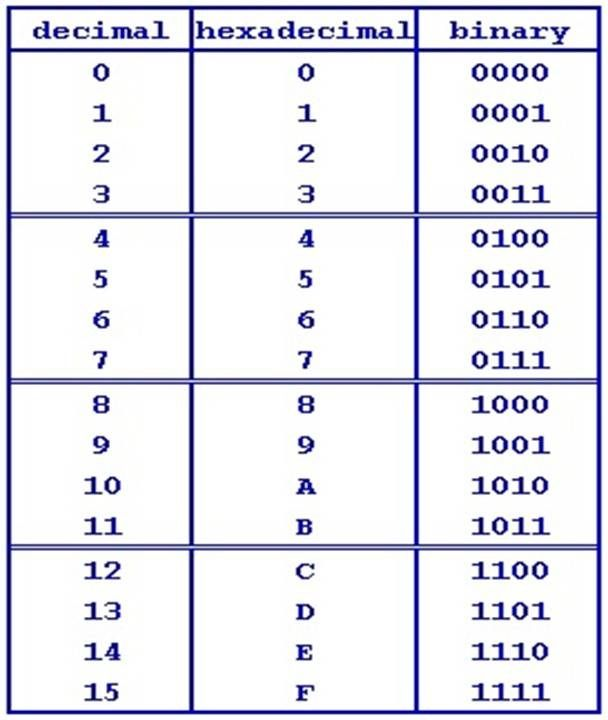
\includegraphics[width=5cm, height=7cm]{june28/table}
\label{conversiontable:1}
\end{center}

From the table above, it becomes clear that a single hexadecimal digit requires four bits for its representation. This matters because it allows us to quickly convert between hexadecimal and binary. Consider, for example, the hexadecimal number $55$. We can look at each hexadecimal digit, and we can write down the corresponding binary number with four bits to obtain $01010101$ as the equivalent binary representation. 


The \verb!printf()! command has a format specifier to print a number in hexadecimal (with the \verb!%X! specifier) or octal (with the \verb!%o! specifier). Moreover, the \verb!%08x! specifier can be used for printing unsigned integers as zero-padded, eight-digit hexadecimal numbers. However, there is no format specifier to print a number in binary. As an example, consider the following code segment: \newpage


\lstset{
caption=Hexadecimal Format Specifier}
\begin{center}
\lstinputlisting[language=c]{june28/june2801.c}\label{Hexadecimal Format Specifier}
\end{center}

The output of this program will be all hexadecimal numbers between $0$ and $32$, inclusive. There are additional zeroes added to the start of each number to ensure that each output is eight digits long. 



So, why do we specify that we want eight bytes, rather than some other number? In our system, an unsigned integer is $4$ bytes, or equivalently, $32$ bits (there are $8$ bits in a byte). Now since each hexadecimal number requires four bits, we require $32/4 = 8$ hexadecimal digits. 

As another example, suppose we're printing out a single character. There is $1$ byte, or equivalently, $8$ bits in a character. Hence, we require $8/4 = 2$ hexadecimal digits to print a character. \\

We can utilize the preceding fact and store a two-digit hexadecimal number as an unsigned character type. 


\subsection{Bitwise Operations}
First, we discuss bit shifting. \\


A bit shift moves each digit in a number's binary representation a specified number of places to the left or right. The left shift operator is written as \verb!<<!, whereas the right shift operator is written as \verb!>>!. The number that directly follows this operator specifies the number of places we wish to shift. 



As a basic example, consider the number $2$, which has binary representation \verb!0011!. If the variable $x$ were storing the value $2$, the statement \verb!x << 1! would return the value $4$ since the binary representation of \verb!x << 1! is \verb!0110! (note that an additional zero has been added at the end). The variable $x$ itself won't be updated from a bitshift. If we want to update the value of \verb!x!, we would have to instead write either \verb!x = x << 1! or \verb!x <<= 1!. Likewise, the statement \verb!x >> 1! would return the value $1$. Performing left and right shifts are equivalent to multiplying or dividing by powers of $2$. That is, a left shift by one multiplies by $2$, and the right shift divides by $2$ (note, however, that they are much faster than multiplying or dividing by $2$).



Some other bitwise operators include the logical operators of \verb!AND, OR, NOT!, and \verb!XOR!. These can be used in C with the binary operators \verb!&, |, ~,! and \verb!^!, respectively. We should already be familiar with these, but to recap, consider the numbers $5$ and $7$. The binary representation of these two numbers are \verb!0101! and \verb!0111!. Consequently, we see that \verb!5 & 7! returns $5$, \verb!5|7! returns $7$, \verb!~5! returns $10$, and \verb!5^7! returns $2$. \\

The identity for the \verb!AND! operator is $0$, and the identity for the \verb!OR! operator is $1$ (i.e. \verb!x&0 = x!, and \verb!x|1 = x!) \\


Note that all of these bitwise operations can also be applied to hexadecimal numbers (or rather, numbers in any base). It's just important to convert everything to binary first.  \\


\subsection{Bitmasking}

Why are bitwise operations important? We can use bitwise operations to perform \vocab{bitmasking}, ultimately allowing us to ``toggle'' or ``retrieve'' bits on and off. 


Consider a function that takes in an integer; say the input is \verb!1010!. If we want to always clear the second bit from the right, this function can simply return the user's input \verb!AND!'d with \verb!1101!, which will always result in a \verb!0! in the second bit. 
As another example, suppose we want to extract the second bit from the right of a given integer. Again, suppose the integer we're working with is \verb!1010!. We can \verb!AND! this number with \verb!0010!, which will clear everything except for our digit of interest. If the result is \verb!0!, the value of that digit is \verb!0!; otherwise, it is \verb!1!. 

Using \verb!AND! in conjunction with right shifts, we can write a program that counts the number of zeroes and ones in the bitwise representation of an integer.

In summary, \begin{itemize}
    \item We can clear bits by \verb!AND'!ing with $0$.
    \item We can check bits by \verb!AND!'ing with $1$.
    \item We can set bits by \verb!OR!'ing with $0$
    \item We can flip bits by \verb!XOR!'ing with $1$. 
\end{itemize}


Consider the following problem that can be solved with bitmasking: Given the hexadecimal number \verb!0xab! (which has binary representation \verb!1010 1011!), perform bitwise operations to make bits in positions $2$ to $4$ (from the left) equal to \verb!110!. 

The solution is to \verb!AND! with \verb!1000 1111! to clear the targeted bit positions, and finally \verb!OR! with \verb!0110 0000! to set them to what we desire. 


\subsection{Big Endian and Little Endian}

\vocab{Endianness} refers to how data is arranged in memory. It is dependent on the hardware we are working on (not the operating system). Endianness is important when we're working at the bit level. 

There are two types of endianness that we are concerned with: \begin{itemize}
    \item In \vocab{Big Endian} refers to how we typically visualize data. In this representation, there's a pointer that points to the most significant byte. 
    \item In \vocab{Little Endian}, the data is laid out in reverse-chronological order, and the pointer points to the least-significant byte.
\end{itemize}


Consider the hexadecimal number \verb!0x01234567!. The following image illustrates how this number would be represented in Big Endian versus Little Endian:

\begin{center}
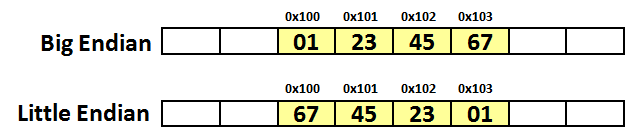
\includegraphics[width=\textwidth, height=4cm]{june28/endianness}
\label{conversiontable:1}
\end{center}

Pretty much, the Little Endian representation is the opposite of what we'd expect. 


Here's a code segment that allows us to determine whether a computer architecture runs in Big Endian or Little Endian



\lstset{
caption=Determining Endianness}
\begin{center}
\lstinputlisting[language=c]{june28/june2802.c}\label{Determining Endianness}
\end{center}

Why are we using a character pointer? Since a character is one byte, iterating with a character pointer allows us to move byte-by-byte through the hexadecimal digits.


Grace runs in Little Endian.
% July
\section{Monday, July 1, 2019}
A \vocab{nibble} is a term used to describe four bits. A very important thing to remember from last lecture is that each hexadecimal digit is represented by a nibble.

\subsection{Unix File Permissions}
% This will be on the exam.
Unix file permissions are based on the octal system. Every file is associated with three entities: the user entity, the group entity, and the ``other'' entity. The user entity describes the file permission of yourself. The group entity describes a set of users on the same system. The ``other'' section describes everyone else. 


The \verb!chmod! command can be used in Unix to change permissions of a file. The general format of the command is \verb!chmod [settings] [file_name]!. What we enter for the \verb![settings]! portion of the command is a three-digit octal number, specifying the permissions for each entity. The first digit corresponds to the specifications for the user, the second digit corresponds to the settings of the group, and the last digit is for the ``other'' entity. 


So, how does it work? We convert each octal digit in \verb![settings]! to a three-digit binary number, which specifies whether the entity has read, write, and/or executing permissions, in that order.


As an example, suppose we execute \verb!chmod 400 a.out!. The corresponding binary representation of \verb!4! is \verb!100!, meaning that the user (the person executing the command) will be able to read the file, but they will not be able to write to the file or execute it. Since the other two octal digits are \verb!0!, the permissions of the group and ``other'' categories aren't modified.



How do we determine what the \verb![settings]! number should be? This is easy - just work backwards. Suppose we want the user and the group to be able to read and execute the file but not write to it. This corresponds to the three-digit binary number \verb!101!, which has octal representation \verb!5!. So, \verb!chmod 550 a.out! does exactly what we want.



We can call \verb!chmod! recursively on a directory using the \verb!-r! flag. 


\subsection{Introduction to Assembly Language}

% \subsubsection{Terminology}

\vocab{Assembly} is a low-level, readable translation of machine language. It is a programming language that we work with when we want to see what the computer is doing. There are many assembly languages out there - in this class, we will use AVR Assembly. We can generate the \verb!.S! file corresponding to the assembly instructions of a \verb!.c! file by compiling with the \verb!-S! flag when using \verb!avr-gcc!. This is not allowed for projects/exercises.



A computer consists of some memory (RAM), and a CPU. Inside of the CPU, there is an \vocab{arithmetic logic unit}, which is responsible for performing computations. Additionally, inside of the CPU, there are \vocab{registers}, which are fast-access locations that instructions use instead of storing all values in memory. Registers are all one byte. In AVR, there are $32$ registers, labeled r0, r1, $\ldots$, r31. A computer also has a \vocab{program counter}, which is a register that specifies the next instruction to be executed. Finally, the computer has an \vocab{immediate}, which consists of constants that are in the instruction itself. 



A program written in AVR assembly has four components to it. Firstly, there are \vocab{instructions}, which specify what the processor will execute. These instructions typically consist of a name, a list of registers, and sometimes a constant value. In addition, there are \vocab{labels}, which represent an address. Labels are typically denoted by some text, followed by a colon. They are also used to define functions. Finally, there are \vocab{assembler directives}, which controls where code and data are placed, as well as \vocab{comments}. \\

How does our assembly code become machine language? We use an \vocab{assembler} (analogous to a compiler) to produce the zeroes and ones associated with our instructions. 

\subsection{An Illustrative Example}

To illustrate how a basic assembly program works, we'll first consider some logically equivalent code written in C:

\lstset{
caption=C Program for Assembly Example
}
\begin{center}
\lstinputlisting[language=c]{july01/july0101.c}
\end{center}

Note that we don't actually use the variable \verb!x! - it's just there so that we can see how to create global variables in assembly. What does this code segment do? It prints the letter \verb!A! (which has ASCII value $65$), and it subsequently prints a newline character (which has ASCII value $10$). \\

The corresponding assembly program is presented below:


%\avrasm{july01/july01}{Hi}

\lstset{
caption=Assembly Example
}
\begin{center}
\lstinputlisting[language={[x86masm]Assembler}]{july01/july0101.asm}
\end{center}

Before we start analyzing this code, it should first be noted that lines beginning with dots are directives, lines ending with colons are labels, lines beginning with a semicolon are comments, and everything else is an instruction.

What observations can we make? 
\begin{itemize}
    \item Comments begin with a single semicolon, but we sometimes prefer to use more semicolons for sylistic reasons.
    \item Symbolic constants are defined with \verb!.set! directive followed by a target text, a comma, and a replacement text. The target text never actually makes it to the machine code; it is processed by the assembler.
    \item By writing the \verb!.data! directive, we indicate that what follows is a data section. We create labels by having some text, followed by a colon. Here, our label is \verb!x!, which stores the memory address of the value $6$. What follows \verb!.byte! indicates the entity being stored at the memory address. This can be written in decimal (as it is), hexadecimal, or even binary. 
    \item The \verb!.text! directive indicates that we're done with our initial setup, and everything that follows is actual code. This is a very important directive to have.
    \item The \verb!.global main! directive allows \verb!main! to be called outside of the current file. Functions, including \verb!main!, begin with labels. Also, functions end with \verb!ret!. 
    \item To call a function, we use the call instruction \verb!call init_serial_stdio!. We will always call this function to permit us to use input and output.
    \item To print the ASCII value of `A,' we need to first load a value into a register using \verb!ldi!. In our program, we move $65$ to register $24$. 
    \item After we load into register $24$, we clear register $25$ with \verb!clr!. Why do we clear register $25$? Because \verb!putchar()! assumes that the value it will display can be found in registers $24$ and $25$. This is a rule defined by gcc. So we clear register $25$ to contain no data.
    \item To flush the buffer, we load in the new line character to register $24$, and we re-clear register $25$ (in case \verb!putchar! messed it up). Finally, we call \verb!putchar! again, and we get our desired output.
    \item The \verb!cli! and \verb!sleep! functions are necessary to stop the program. 
\end{itemize}










Side-note: we can't have floating-point types in AVR Assembly, but we can have integers, characters, and strings. 
\section{Tuesday, July 2, 2019}
No discussion today. Today is day two of Assembly.


\subsection{Data Space Instructions}

In order to transfer the contents of a register back into memory (like a variable), we can use the \verb!sts! instruction, which is short for ``store to data space.'' Using \verb!sts! in assembly is analogous to assigning a variable some value. On the other hand, we can use stored memory to write to a register using the \verb!lds! instruction, which is short for ``load direct from data space.'' The general syntax for \verb!sts! is \verb!sts [data destination], [register source]!. The general syntax for \verb!lds! is \verb!lds [register destination], [data source]!. 

Another useful instruction is \verb!inc!, which simply increments the contents of a register. As we'd expect, the syntax for this instruction is just \verb!inc [register name]!.


Consider the following code segment, which illustrates all three of these instructions:


\lstset{language=[x64]Assembler}
\lstset{
caption=Storing and Loading to Data Spaces
}
\begin{lstlisting}
;;; Global data
    .data
a:  .byte 0x2
b:  .byte 0b00000100
c:  .byte 0

;;; Program code
    .text

.global main
main:

    call init_serial_stdio
    lds     r18, a ; stores contents of a into r18.
    lds     r19, b ; stores contents of b into r19.
    push    r19 ; saves value of r19 on the stack.
    add     r19, r18 ; adds contents of registers.
    sts     c, r19 ; stores contents of r19 into c.
    
    lds r18, c ; stores contents of c into r19.
    inc r18 ; increments r18
    pop r19 ; restores r19
    inc r19 ; increments r19
    
    cli ; stops the program
\end{lstlisting}


What's happening here?

On Lines $3, 4,$ and $5$, we're just declaring three global variables: \verb!a!, \verb!b!, and \verb!c!. Like we saw yesterday, the \verb!.data! directive indicates that we're starting our data section, and the \verb!.byte! directive indicates that the value that follows should be stored in the specified variable. In this case, we store \verb!0x2! (hexadecimal for $2$) in \verb!a!, $100$ (binary for $4$) in \verb!b!, and $0$ in \verb!c!. The reason why we're using different base systems is just to clearly convey that it is allowed. 

All of our variables have been initialized, so we can begin writing our code (officially, this is indicated by the \verb!.text! directive on Line $8$). In our main, we see an example of \verb!lds! in action: the instruction takes a register and some data, and it loads the contents of the data into the register. In this case, \verb!r18! stores \verb!2!, and \verb!r19! stores \verb!4!. The contents of \verb!r19! are pushed onto the stack for safekeeping. 


The \verb!add! instruction on Line $17$ stores the contents of \verb!r19! and \verb!r18! and stores the sum in \verb!r19! (it overwrites the previous value, which is precisely why we pushed the original value onto the stack). On Line $18$, the \verb!sts! instruction is used to store the sum into variable \verb!c!. This value is incremented by one, the original contents of \verb!r19! are restored, and the contents of \verb!r19! are incremented by one. The final value stored in \verb!r18! is $7$. 



\subsection{Instructions List}

The list below summarizes some important instructions that we should become familiar with (we've already seen some of these): \begin{itemize}
    \item \verb!ldi! initializes a register with a constant value. Its general syntax is \verb!ldi [register] [constant]!. For instance, \verb!ldi r24, 5! would set the contents of \verb!r24! to $5$. 
    \item \verb!lds! loads data from memory into a register --- we saw this in the previous example.
    \item \verb!sts! stores data from a register into memory --- we also saw this in the previous example.
    \item \verb!clr! clears the contents of a register. Its general syntax is \verb!clr [register]!. After this instruction is executed, the contents of the register it was performed on becomes $0$.
    \item \verb!add! is used to add the contents of two registers. Its general syntax is \verb!add [register1], [register2]!. After this instruction is executed, the contents of \verb!register1! are replaced with \verb!register1 + register2!. 
    \item \verb!inc! is used to increment the value of a register by one. We saw this in the previous example. 
    \item \verb!push! is used to push a register value onto the stack. Its syntax is \verb!push [register]!. 
    \item \verb!pop! is used to move data from the top of the stack into another register. Its syntax is \verb!pop [register]!. Note that you don't have to pop to the same register that was pushed. There should be a one-to-one correspondence between \verb!pop! and \verb!push! instructions.
    \item \verb!call! is used to call a function, as we saw with the putchar example yesterday.
    \item \verb!ret! is used to return from a function.
    \item \verb!nop! is short for ``no operation,'' and it does nothing. Why does it exist? To make our processor wait and do nothing.
    \item \verb!mov! has syntax \verb!mov [destination register], [source register]!. It copies the contents of \verb!source register! into \verb!destination register!. Note that the name ``move'' is slightly misleading here - the contents of \verb!source register! aren't moving anywhere - they are being copied, not moved.
\end{itemize}

\subsection{Caller/Callee Saving}

The $32$ registers that we use in Assembly are all global registers. What this means is that these registers are shared among every function, including the main. To illustrate why this matters, suppose we were to store $20$ in register \verb!r19! in the main. We then decide to call some function, which stores $100$ in the register \verb!r19! as a part of its processing. This change will also be reflected in the main (and everywhere else in the program). 

Registers are shared across the entire program, which makes things more complicated. How can we avoid overwriting registers used by functions? The solution to this problem comes from two protocols that we use: \begin{enumerate}
    \item \vocab{Caller-saved protocol}: When writing a function, we assume the programmer who called the function has already saved the contents of registers from \verb!r18! to \verb!r27!, \verb!r30!, and \verb!r31!. So, the function writer should be operating on only these registers, and it's up to the programmer to have already saved anything of importance in these registers. We are expected to only operate on these registers when writing our functions as well.
    \item \vocab{Callee-saved protocol}: If a function writer wants to use registers \verb!r2! to \verb!r17!, \verb!r28!, or \verb!r29! inside of their function, they need to be saving the registers prior to using them. Furthermore, the contents of these registers need to be restored back to their original values before leaving the function.
\end{enumerate}

What do these protocols mean to us? It means that there is less work for both the function writer and the function caller. On one hand, the function writer can use several registers without worrying about overwriting important data. On the other hand, the function caller has a set of registers where they can store data and call a function with certainty that their data will not be overriden. \\

To better understand these two protocols, consider a blackboard that is shared among different professors. The blackboard follows the caller-saved protocol: a professor who enters the classroom to teach is allowed to erase whatever is on the blackboard. It is assumed that any important information on the blackboard has already been recorded by the previous user. On the other hand, if the blackboard were callee-saved, the most recent user would have to restore the blackboard to however it originally was, prior to their use.  


We can use the fact that registers are shared across the entire program to pass and return values to functions.

\subsection{Arguments and Return Values}

Unlike C, Assembly doesn't have function headers: a function declaration is just a label. So, how do we take in arguments and/or return values? Both of these tasks are accomplished through registers. If we have a lot of arguments or return values and we run out of registers, we can use the stack (but we won't need to worry about that). 



When we're passing arguments to a function, we can just load the argument into a register for the function to use. Arguments are aligned to start in even-numbered registers, beginning at \verb!r24! and going downwards. Also, if we're passing an odd number of parameters, there will always be one free register above them. So, for instance, if we're passing in a single \verb!char! to a function, we would load the value of that character into \verb!r24!, and we would leave \verb!r25! empty as there is an odd number of parameters.

The conventions for passing arguments to functions are illustrated below:
\begin{itemize}
    \item If we're passing an argument that's just one byte, the argument will go in \verb!r24! and \verb!r25! will be cleared.
    \item If we're passing an argument that's two bytes, the arguments will go in \verb!r24! and \verb!r25! (note how there is no free register since there are two arguments). 
    \item If we're passing four bytes of arguments, the arguments will go in \verb!r25, r24, r23, r22!, and there won't be any empty registers.  
\end{itemize} 

Once these registers have been loaded with the arguments, we can use the \verb!call! instruction to go inside of the function. The function will share the contents of these registers, and it will be able to perform any necessary processing. 



How do we return values from functions? It's the same idea as passing arguments. The exact same convention for passing parameters. For instance, if the function returns one byte, the return value is loaded into register \verb!r24!. 


Note that the conventions for passing arguments and returning values align with the caller/callee-saved protocol. Particularly, we are passing parameters through caller-saved registers. The function caller is expected to have already saved any important data in these registers, as the function will be changing the contents of these registers after processing.


After introducing these concepts, let's look at an example that's very similar to what we saw yesterday:


\lstset{
caption=Assembly: Arguments and Return Values
}
\begin{lstlisting}
    .text
    
.global main
main:
    call init_serial_stdio
    
    ; Printing 'A'
    clr r25
    ldi r24, 65
    call putchar
    
    cli
    sleep
\end{lstlisting}


The function \verb!putchar! from C takes in a single character as an argument. To pass in the argument `A,' we clear register \verb!r25! and load the ASCII value of `A' into \verb!r24!. This aligns with the convention we've previously discussed. Finally, we call \verb!putchar!, which is now free to do whatever it desires with these parameters. It will no longer be guaranteed that register \verb!r24! and \verb!r25! are how they were prior to the function call.



\subsection{Accessing Memory}

In Assembly, \verb!lo8! and \verb!hi8! can be used to extract the lower and higher $8$ bits of data (if we are passing in $2$ bytes of data, there will be two $8$ bit blocks). The instruction \verb!ldi r24, lo8(x)! would load the lower byte of variable \verb!x! into register \verb!r24!. 



We have already seen that \verb!lds! and \verb!sts! are instructions that allow us to read and write to memory. Assembly has three pairs of registers that allow us to access memory. These pairs of registers are called \verb!X! (resides in registers \verb!r26! and \verb!r27!), \verb!Y! (resides in registers \verb!r28! and \verb!r29!), and \verb!Z! (resides in registers \verb!r30! and \verb!r31!). 


\verb!X!, \verb!Y!, and \verb!Z! represent addresses in memory (like pointers). Conventionally, the low byte is stored in the even-numbered register, and the high byte is stored in the odd-numbered register. 


Consider the following example:

\begin{lstlisting}
    .data
pctd: 
    .asciz  "%d "

values:
    .byte   15
    .byte   16
    .byte   17
    .byte   18
    
    .text

.global main
main:

    call init_serial_stdio
    
    lds r24, values
    clr r25
    call pint
    ldi r24, 10
    clr r25
    call putchar
    
    ldi r26, lo8(values)
    ldi r27, hi8(values)
    ld r24, X
    push r26 ; Caller-save
    push r27
    clr r25
    ldi r24, 10
    clr r25
    call putchar
    
    pop r27
    pop r26
    adiw r26, 1 ; Move the pointer
    
    ld r24, X
    clr r25
    call pint
    ldi r24, 10
    clr r25
    call putchar
    
    cli ; Terminate program
    sleep 
    ret
\end{lstlisting}

First off, the label \verb!values! is defined differently than what we've seen so far: there are multiple \verb!.byte! directives in its definition. The key thing to remember here is that a label is just an address in memory. Hence, one way we can interpret \verb!values! is the value $15$: if we were to load this value somewhere, the value $15$ would be loaded. We can alternatively interpret \verb!values! as the name of an array with contents $15, 16, 17$, and $18$.


When we call \verb!pint! (the function for printing), $15$ is outputted. We then load the ASCII value for a new line, and we call \verb!putchar! to print a new line. 

On Lines $25$ and $26$, we load the low byte and high bytes of \verb!values! into the registers \verb!r26!, and \verb!r27!. The registers \verb!r26! and \verb!r27! are special: they represent a register pointer, denoted by \verb!X!. Hence, on the subsequent line, we can use \verb!ld! to initialize \verb!r24! to whatever \verb!X! points to (note that we use \verb!ld! for register pointers instead of \verb!lds!). Finally, when we call \verb!pint! again, $15$ is printed again (as \verb!r24! now points to \verb!X!).

Okay, now what if we want to print the other values in the array? We use pointer arithmetic, just like in C. The \verb!adiw! instruction is short for ``add immediate to word',' and it has syntax \verb!adiw [register], [number]!, and it increments the contents of \verb![register]! by \verb![number]!. This is exactly what's happening from Lines $37$ to $44$. These lines increment \verb!X! and print \verb!16! along with a new line character.


Tomorrow, we will pick up from this point and do more Assembly.



\end{document}